\documentclass[11pt]{report}
% define the title
\usepackage[brazil]{babel}
\usepackage[utf8]{inputenc}		%Usar acentos diretos do teclado
\usepackage[T1]{fontenc}		%Padrão para imagens
\usepackage{graphicx}
\usepackage{subfigure}
\usepackage{rotating}
\usepackage{longtable}
\usepackage{amsmath}
\usepackage{amsfonts}
\usepackage{amssymb}
\usepackage{geometry}
\usepackage{caption}
\geometry{left=3cm, right=2cm, top=2cm, bottom=2cm}
% Title Page
\title{Trabalhos 1, 2 e 4 - Comunicação Digital}
\author{Pedro Yochinori Gushiken}



\begin{document}
\maketitle
\tableofcontents
\chapter{Trabalho 1 - Comentários sobre ADPCM e Modulação Delta em comparação com DPCM e PCM}
\section{Modulação Delta}
\subsection{Comentários}
Na modulação Delta, a mensagem é super amostrada (numa taxa muito superior a Nyquist), aumentando a correlação entre amostras adjacentes do sinal. Isto permite o uso de uma estratégia de quantização simples. Na forma mais básica de modulação Delta a diferença entre uma amostra e a outra é quantizada através de apenas um bit e a aproximação do sinal é construída fazendo um incremento de $\pm \Delta$, a depender da aproximação estar acima ou abaixo do nível do sinal amostrado (erro quantizado, multiplicado por delta e integrado discretamente ao longo de cada período). Quando o $\Delta$ usado é fixo está estratégia é chamada de modulação Delta linear. Este esquema é chamado no Haykin de DPCM com preditor de nível 0.\\

A maior virtude da modulação Delta é sua simplicidade de implementação.\\ 

Quanto ao ruído de quantização, este esquema sofre de dois tipos:\\ 
1) "Sobrecarga de Inclinação"(slope overload), onde o $\Delta$ escolhido é pequeno demais para um determinado trecho do sinal onde a inclinação excede um certo valor e mesmo com o sinal do erro quantizado sendo constante num determinado intervalo a aproximação não é capaz de acompanhar o sinal. Este ruído também ocorre na modulação PCM diferencial.\\
2)"Ruído Granular"(Granular Noise), que é análogo ao ruído de quantização no PCM. É gerado quando a inclinação da reta é baixa. No caso de um $\Delta$ fixo, a aproximação sempre terá uma certa diferença em relação ao sinal amostrado. Isso pode ser claramente ilustrado caso se gere um sinal amostrado que é constante num determinado intervalo, neste caso o erro quantizado tenderá a uma sequência alternando constantemente entre +1 e -1. 

\subsection{Implementação}
Foi feita uma implementação simples de modulação Delta linear, o sinal amostrado contém quatro componentes senoidais com w=200 até 50 rad/s em incrementos de 50 radianos/s. O clock usado na amostragem é de 10kHz, que cumpre o requerimento de super amostragem. O filtro passa-baixa usado é de terceira ordem. O valor de $\Delta$ é de 0.05.

\begin{figure}
\centering
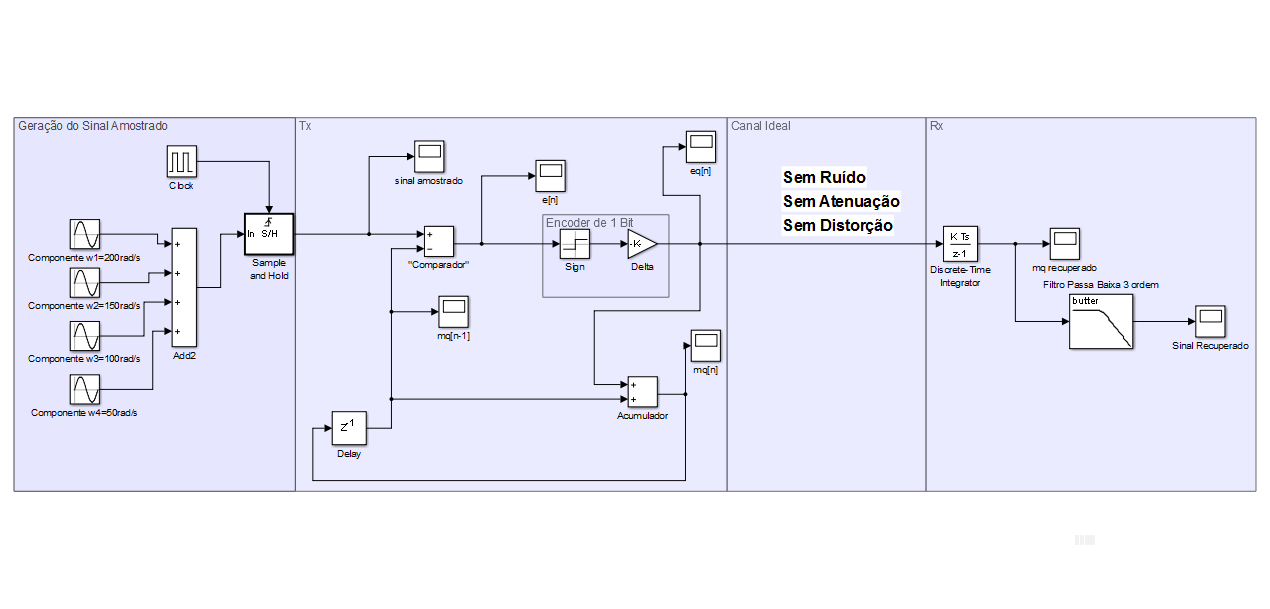
\includegraphics[width = 16 cm, height = 8 cm]{EsquemaModDelta.png}
\caption{Esquema usado para implementação da Modulação Delta}
\end{figure}

\begin{figure}
\centering
\begin{minipage}{.5\textwidth}
  \centering
  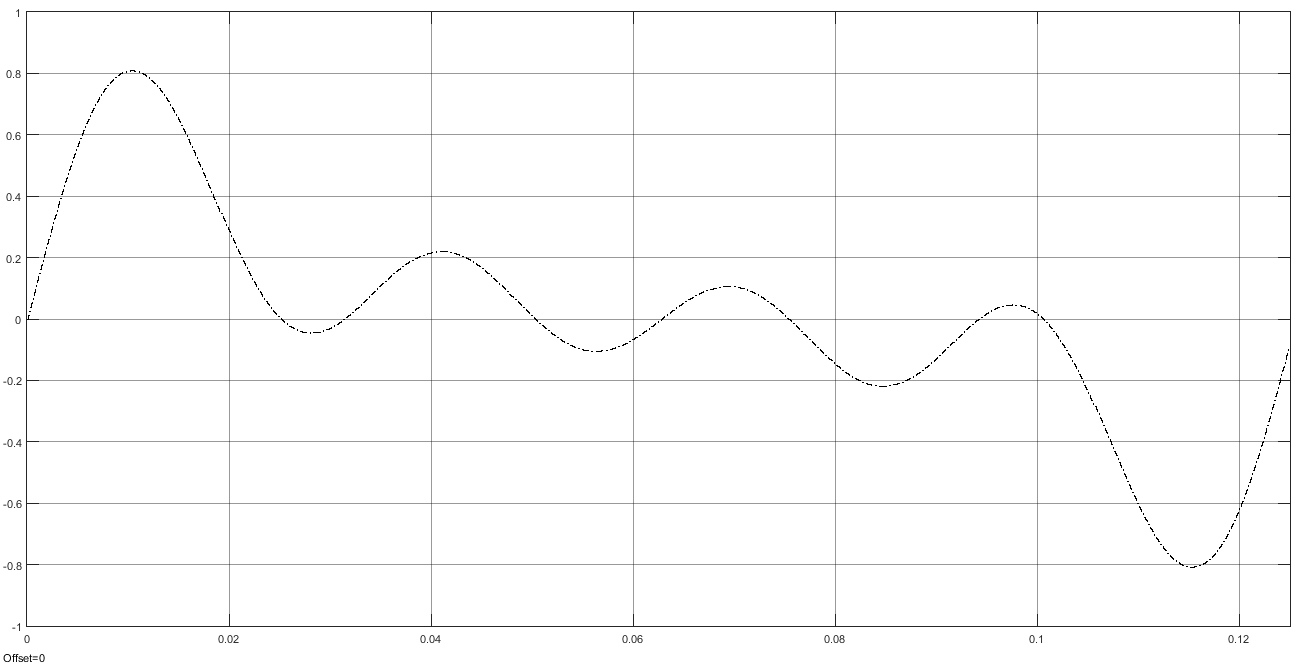
\includegraphics[width=\linewidth]{SinalAmostradoModDelta.png}
  \captionof{figure}{Sinal super amostrado}
  \label{fig:test1}
\end{minipage}%
\begin{minipage}{.5\textwidth}
  \centering
  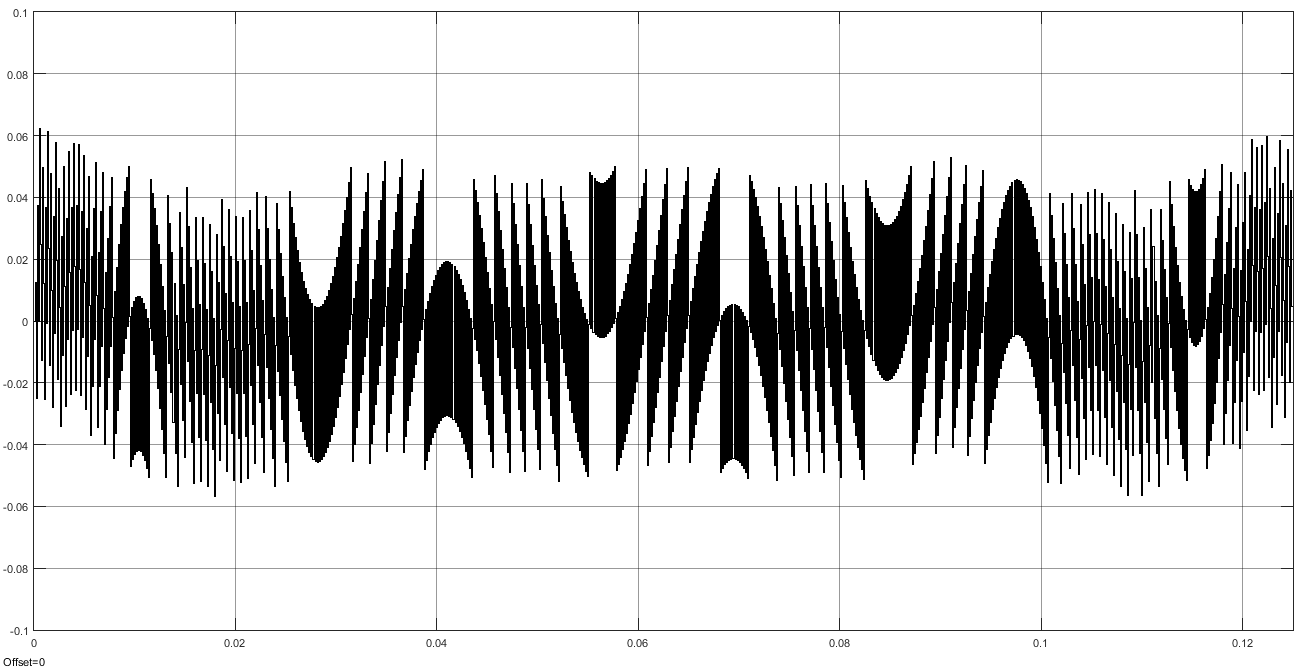
\includegraphics[width=\linewidth]{EnModDelta.png}
  \captionof{figure}{Erro e[n] entre o sinal amostrado e a aproximação do sinal $m_q[n]$}
  \label{fig:test2}
\end{minipage}
\end{figure}

\begin{figure}
\centering
\begin{minipage}{.5\textwidth}
  \centering
  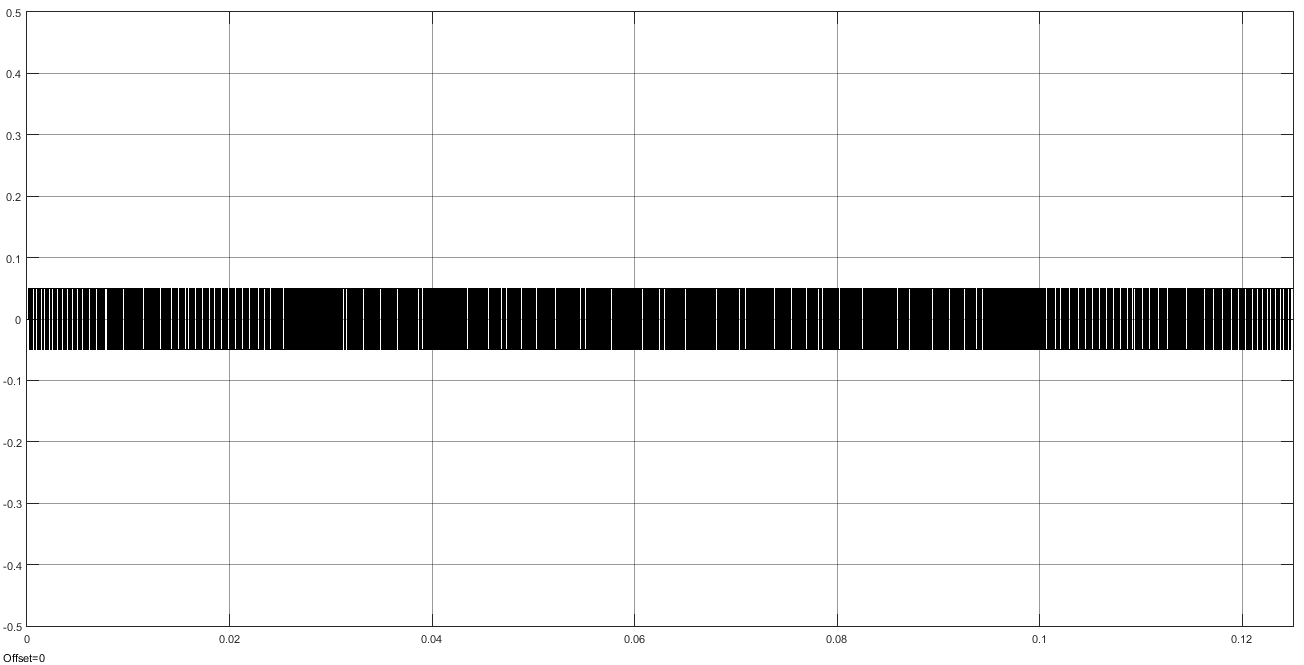
\includegraphics[width=\linewidth]{EqnModDelta.png}
  \captionof{figure}{Erro e[n] quantizado e multiplicado por $\Delta$}
  \label{fig:test3}
\end{minipage}%
\begin{minipage}{.5\textwidth}
  \centering
  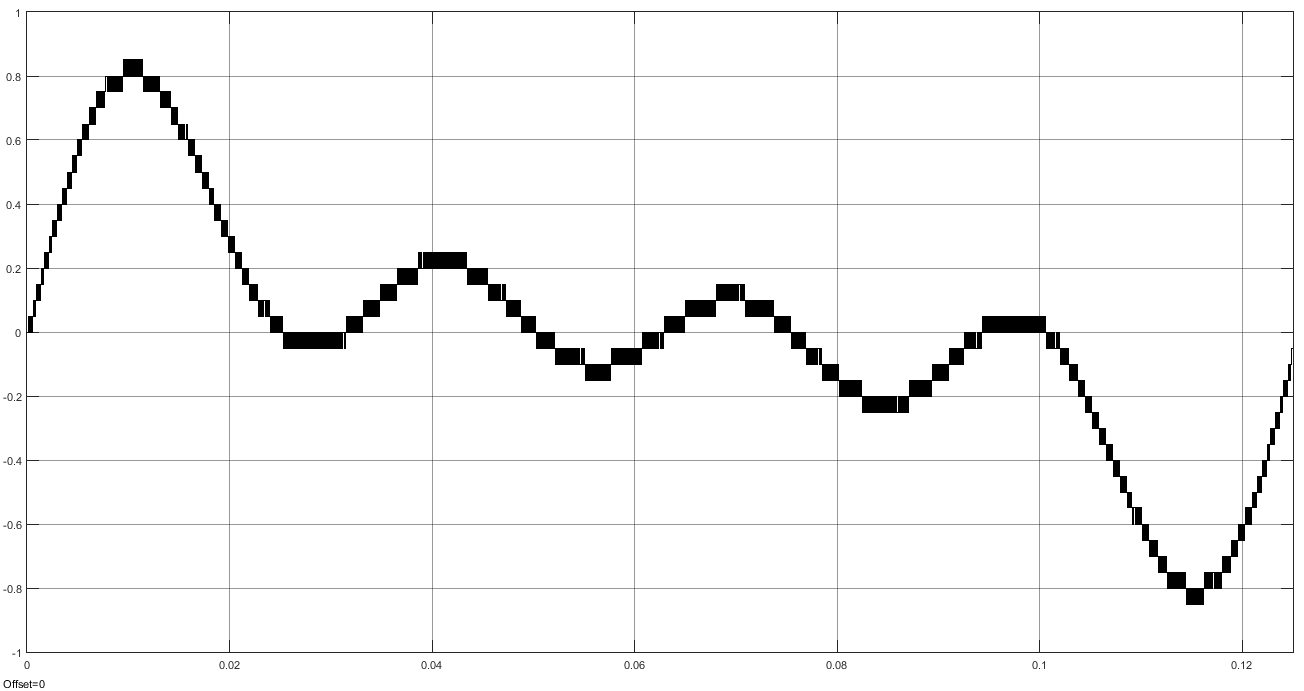
\includegraphics[width=\linewidth]{MqModDelta.png}
  \captionof{figure}{Aproximação do sinal $m_q[n]$}
  \label{fig:test4}
\end{minipage}
\end{figure}

\begin{figure}
\centering
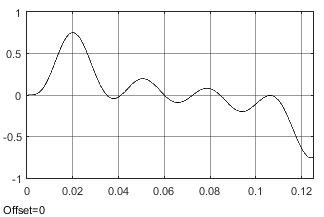
\includegraphics{SinalRecuperadoModDelta.png}
\caption{Sinal Recuperado}
\end{figure}

\section{ADPCM}
\subsection{Comentários}
O uso do PCM tradicional à uma taxa de transmissão de 64kbps para voz em muitas aplicações se torna muito custoso do ponto de vista do consumo de banda. Neste tipo de aplicação se torna necessário a codificação para atingir taxas de bit menores enquanto são mantidas a fidelidade e qualidade do áudio. Se torna necessário então o uso de um codificador de forma de onda, cuja filosofia de design tem em mente dois objetivos claros:\\

\noindent1)Remoção de redundâncias na representação do sinal.\\
2)Assinalar os bits disponíveis para as partes não redundantes do sinal de uma forma eficiente.\\

No caso do ADPCM, é possível reduzir a taxa de bits necessária para manter a mesma qualidade para 32kbps, através do uso de predição e quantização adaptativas. A modulação PCM Diferencial Adaptativa se aproveita do fato de que os sinais transmitidos geralmente tem uma característica não estacionária, isto é, a variância do sinal e autocorrelação mudam de acordo com o tempo. Este fato torna possível implementar um valor de passo para a quantização que muda de acordo com o tempo e estimativa da variância do sinal, assim como alterar os coeficientes do preditor de forma a melhor se ajustar ao sinal. 
\section{Tabela Comparativa}

\begin{table}[htbp]
  \centering
    \caption{Tabela de comparação qualitativa dos esquemas de modulação estudados}
    \begin{tabular}{ccccc}
    \textbf{Parâmetro} & \textbf{PCM} & \textbf{DPCM} & \textbf{ADPCM} & \textbf{Modulação Delta}\\
    Consumo de Banda     & Médio &  Baixo & Muito Baixo & Baixo \\
    Complexidade de Implementação     & Baixa & Média   & Alta & Muito Baixa  \\
    Ruído de Quantização     & Alto & Baixo   & Muito Baixo & Médio\\     
    \end{tabular}%

\end{table}

\section{Uso Comercial}

O ADPCM em 32kbps é aceito como um padrão internacional para transmissão de voz em conjunto com o PCM a 64kbps. Não foram encontradas aplicações comerciais da modulação Delta linear ou suas variantes na pesquisa (o que não quer dizer que não existam). 

\chapter{Trabalho 2 - Código Comentado do Diagrama de Olho}
\section{Comentários sobre o Código}
\begin{verbatim}
%(pnrz.m)
%Geração de um pulso retangular de largura T
%Uso da função: pout=pnrz(T);
%definição da função
function pout=prect(T);
%pout é um vetor de 1's de tamanho T
pout = ones(1,T);
end

%(prz.m)
%Geração de um pulso retangular de largura T/2
%Uso da função: pout = prz(T);
%definição da função:
function pout=prz(T);
%pout é um vetor com T/4 zeros, seguido de T/2 1's, seguido de T/4 zeros
pout = [zeros(1,T/4) ones(1, T/2) zeros(1, T/4)];
end

%(psine.m)
%geração de um pulso senoidal de largura T
%definição da função:
function pout=psine(T)
%pout é um vetor igual ao seno de pi*(T de 0 a T-1)/T
pout = sin(pi*[0:T-1]/T);
end

%(prcos.m)
%Uso: y=prcos(rollfac,lenght,T)
%definição da função:
function y=prcos(rollfac,lenght, T)
%rollfac = 0 a 1 é o fator de roll off
%lenght é a largura onesided do pulso no número de T
%lenght = 2T + 1;
%T é a taxa de sobreamostragem
%rcosfir gera um filtro de cosseno levantado de acordo com os argumentos
y=rcosfir(rollfac,lenght,T,1,'normal');
end

%(binary_eye.m)
%Geração e Plotagem de Diagramas de Olho
%limpar as variáveis e a tela atual de figura
clear;clf;
data = sign(randn(1,400)); % gerar 400 bits randomizados

%geração de 400 pontos de ruído com variância r
%r = 0.01;
%ruid = randn(1,400)*sqrt(r);
%data = data + ruid

Tau = 64; %definir o período de símbolo
% gerar trem de impulsos inserindo Tau-1 zeros entre cada bit
dataup = upsample(data, Tau) 
yrz = conv(dataup, prz(Tau)); %Sinal polar RZ, conv é a operação convolução
yrz = yrz(1:end-Tau+1); %retirar a "cauda" do vetor yrz
ynrz = conv(dataup, pnrz(Tau)); %Sinal polar NRZ
ynrz = ynrz(1:end-Tau+1); %Retirar a "cauda" do vetor ynrz
ysine = conv(dataup,psine(Tau)); %Meia Senóide Polar
ysine = ysine(1:end-Tau+1); %Retirar a "cauda" do vetor ysine
Td=4; %definição de Td
yrcos=conv(dataup, prcos(0.5,Td,Tau)); 

%cosseno levantado truncado em 4 períodos com rolloff =0.5
yrcos=yrcos(2*Td*Tau:end-2*Td*Tau+1); %Gerando trem de pulsos

%geração do diagama de olho RZ
eye1=eyediagram(yrz,2*Tau,Tau,Tau/2); title('RZ eye-diagram'); 

%geração do diagrama de olho NRZ
eye2=eyediagram(ynrz,2*Tau,Tau,Tau/2); title('NRZ eye-diagram'); 

%geração do diagrama de olho Meia-Senóide
eye3=eyediagram(ysine, 2*Tau, Tau, Tau/2); title=('Half-Sine eye-diagram'); 

%geração do diagrama de olho Cosseno-Levantado
eye4=eyediagram(yrcos,2*Tau,Tau); title('Raised-Cosine eye-diagram');

%(Mary_eye.m)
%Geração de Diagrama de Olho e Plotagem (PAM Quaternário)
%limpar as variáveis e telas de figura
clear;clf;
%geração de 400 símbolos PAM quaternário (valores possíveis: -1,-3, 1, 3) 
data = sign(randn(1,400)) +2*sign(randn(1,400));

%geração de 400 pontos de ruído com variância r
%r = 0.01;
%ruid = randn(1,400)*sqrt(r);
%data = data + ruid

%definição do período de símbolo
Tau=64;
% gerar trem de impulsos inserindo Tau-1 zeros entre cada bit
dataup = upsample(data, Tau) 
yrz = conv(dataup, prz(Tau)); %Sinal polar RZ, conv é a operação convolução
yrz = yrz(1:end-Tau+1); %retirar a "cauda" do vetor yrz
ynrz = conv(dataup, pnrz(Tau)); %Sinal polar NRZ
ynrz = ynrz(1:end-Tau+1); %Retirar a "cauda" do vetor ynrz
ysine = conv(dataup,psine(Tau)); %Meia Senóide Polar
ysine = ysine(1:end-Tau+1); %Retirar a "cauda" do vetor ysine
Td=4; %definição de Td
yrcos=conv(dataup, prcos(0.5,Td,Tau)); 

%cosseno levantado truncado em 4 períodos com rolloff =0.5
yrcos=yrcos(2*Td*Tau:end-2*Td*Tau+1); %Gerando trem de pulsos

%geração do diagama de olho RZ
eye1=eyediagram(yrz,2*Tau,Tau,Tau/2); title('RZ eye-diagram'); 

%geração do diagrama de olho NRZ
eye2=eyediagram(ynrz,2*Tau,Tau,Tau/2); title('NRZ eye-diagram'); 

%geração do diagrama de olho Meia-Senóide
eye3=eyediagram(ysine, 2*Tau, Tau, Tau/2); title=('Half-Sine eye-diagram'); 

%geração do diagrama de olho Cosseno-Levantado
eye4=eyediagram(yrcos,2*Tau,Tau); title('Raised-Cosine eye-diagram');

\end{verbatim}

\section{Degradações}
\subsection{Ruído Branco}
O ruído branco AWGN pode ser gerado simplesmente através da função randn(), que gera uma distribuição normal, podemos gerar um vetor R=randn(1,400)*sqrt(r), adicionando este vetor ao vetor de dados gerado podemos enxergar qual a contribuição do ruído no diagrama de olho para um determinado r, que é a variância, neste caso escolhemos r=0.01 de forma a não fechar completamente o diagrama, mas ainda mostrar um pouco do "fechamento".
\section{Diagramas de olho}
\pagebreak


\begin{figure}
\centering
\begin{minipage}{.5\textwidth}
  \centering
  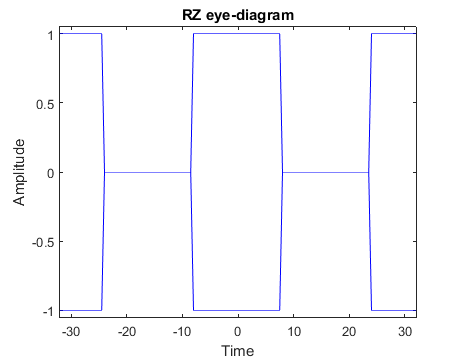
\includegraphics[width=\linewidth]{DolhoRZsrb.png}
  \captionof{figure}{RZ Binário sem ruído}
  \label{fig:test5}
\end{minipage}%
\begin{minipage}{.5\textwidth}
  \centering
  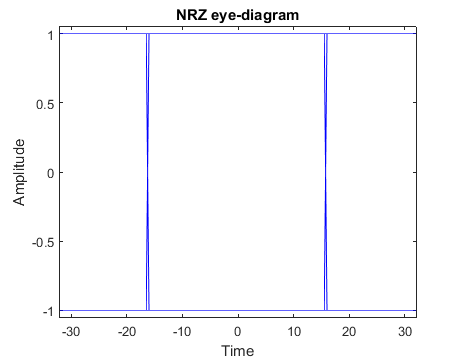
\includegraphics[width=\linewidth]{DolhoNRZsrb.png}
  \captionof{figure}{NRZ Binário sem ruído}
  \label{fig:test6}
\end{minipage}
\end{figure}

\begin{figure}
\centering
\begin{minipage}{.5\textwidth}
  \centering
  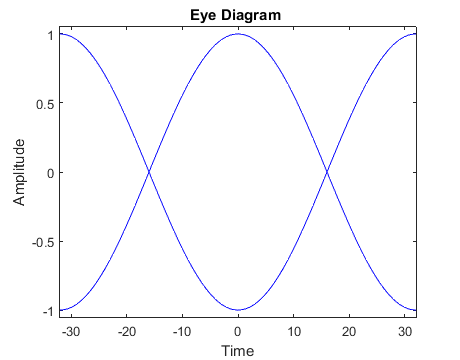
\includegraphics[width=\linewidth]{Dolhosensrb.png}
  \captionof{figure}{Meia Senóide Binário sem ruído}
  \label{fig:test7}
\end{minipage}%
\begin{minipage}{.5\textwidth}
  \centering
  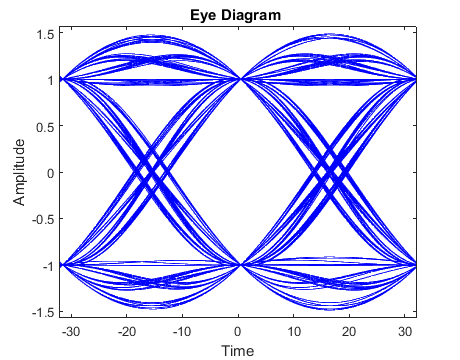
\includegraphics[width=\linewidth]{Dolhoclsrb.png}
  \captionof{figure}{Cosseno Levantado Binário sem ruído}
  \label{fig:test8}
\end{minipage}
\end{figure}


\begin{figure}
\centering
\begin{minipage}{.5\textwidth}
  \centering
  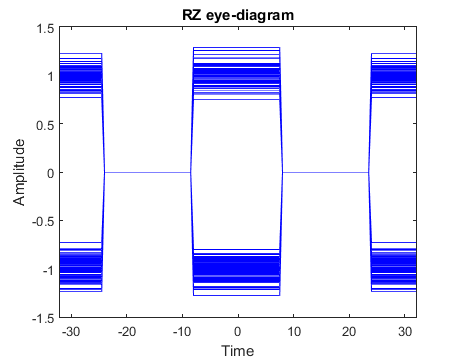
\includegraphics[width=\linewidth]{DolhoRZcrb.png}
  \captionof{figure}{RZ Binário com ruído}
  \label{fig:test9}
\end{minipage}%
\begin{minipage}{.5\textwidth}
  \centering
  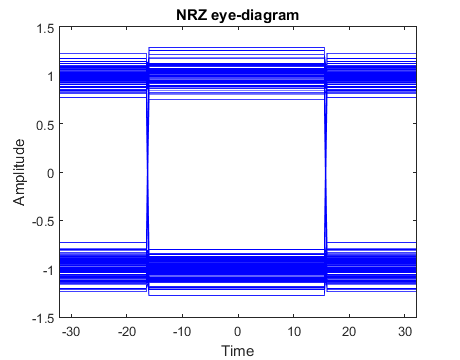
\includegraphics[width=\linewidth]{DolhoNRZcrb.png}
  \captionof{figure}{NRZ Binário com ruído}
  \label{fig:test10}
\end{minipage}
\end{figure}

\begin{figure}
\centering
\begin{minipage}{.5\textwidth}
  \centering
  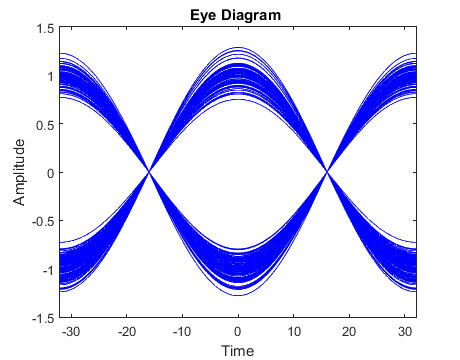
\includegraphics[width=\linewidth]{Dolhosencrb.png}
  \captionof{figure}{Meia Senóide Binário com ruído}
  \label{fig:test11}
\end{minipage}%
\begin{minipage}{.5\textwidth}
  \centering
  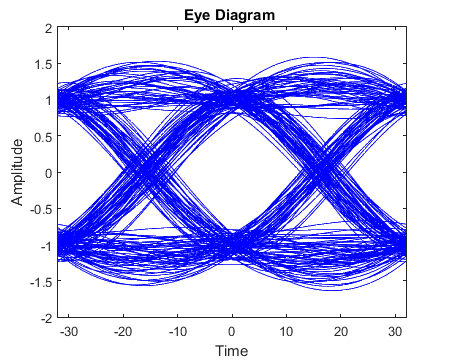
\includegraphics[width=\linewidth]{Dolhoclcrb.png}
  \captionof{figure}{Cosseno Levantado Binário com ruído}
  \label{fig:test12}
\end{minipage}
\end{figure}


\begin{figure}
\centering
\begin{minipage}{.5\textwidth}
  \centering
  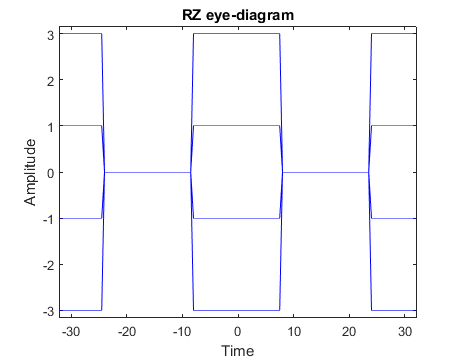
\includegraphics[width=\linewidth]{DolhoRZsrq.png}
  \captionof{figure}{RZ Quaternário sem ruído}
  \label{fig:test13}
\end{minipage}%
\begin{minipage}{.5\textwidth}
  \centering
  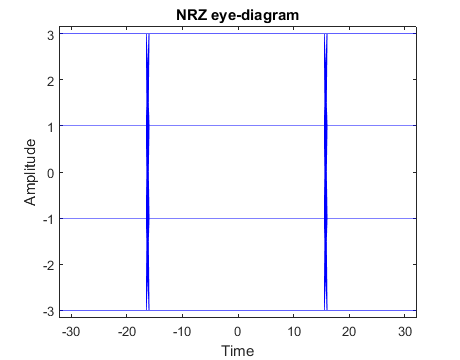
\includegraphics[width=\linewidth]{DolhoNRZsrq.png}
  \captionof{figure}{NRZ Quaternário sem ruído}
  \label{fig:test14}
\end{minipage}
\end{figure}

\begin{figure}
\centering
\begin{minipage}{.5\textwidth}
  \centering
  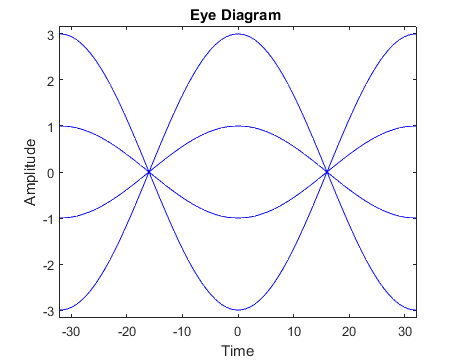
\includegraphics[width=\linewidth]{Dolhosensrq.png}
  \captionof{figure}{Meia Senóide Quaternário sem ruído}
  \label{fig:test15}
\end{minipage}%
\begin{minipage}{.5\textwidth}
  \centering
  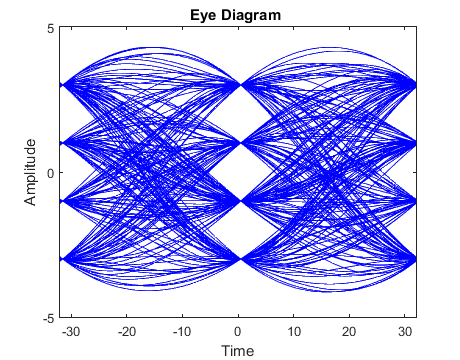
\includegraphics[width=\linewidth]{Dolhoclsrq.png}
  \captionof{figure}{Cosseno Levantado Quaternário sem ruído}
  \label{fig:test16}
\end{minipage}
\end{figure}


\begin{figure}
\centering
\begin{minipage}{.5\textwidth}
  \centering
  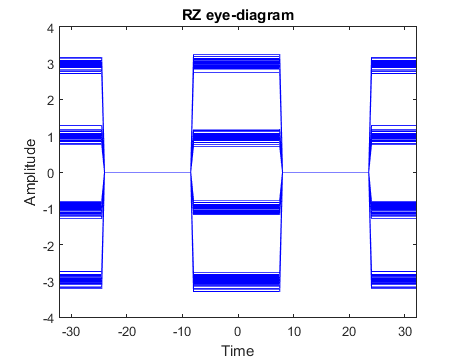
\includegraphics[width=\linewidth]{DolhoRZcrq.png}
  \captionof{figure}{RZ Quaternário com ruído}
  \label{fig:test17}
\end{minipage}%
\begin{minipage}{.5\textwidth}
  \centering
  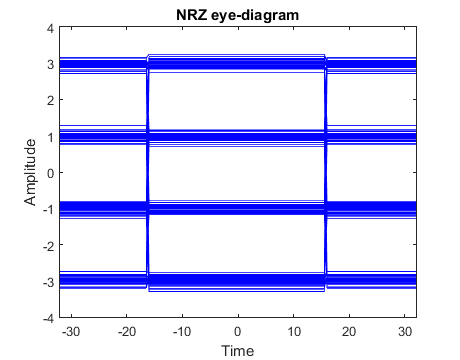
\includegraphics[width=\linewidth]{DolhoNRZcrq.png}
  \captionof{figure}{NRZ Quaternário com ruído}
  \label{fig:test18}
\end{minipage}
\end{figure}

\begin{figure}
\centering
\begin{minipage}{.5\textwidth}
  \centering
  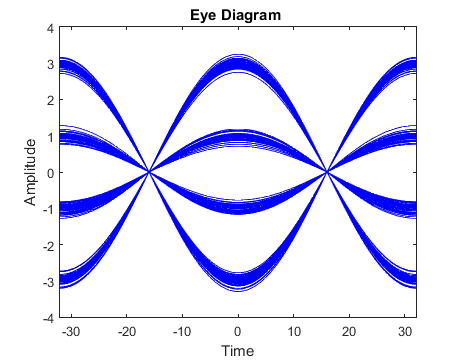
\includegraphics[width=\linewidth]{Dolhosencrq.png}
  \captionof{figure}{Meia Senóide Quaternário com ruído}
  \label{fig:test19}
\end{minipage}%
\begin{minipage}{.5\textwidth}
  \centering
  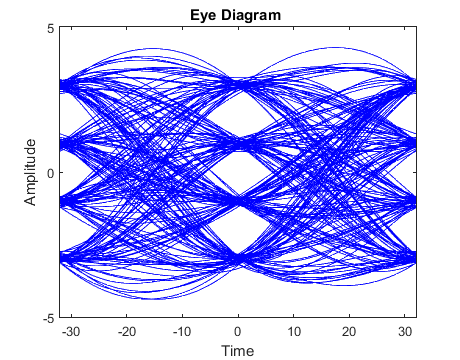
\includegraphics[width=\linewidth]{Dolhoclcrq.png}
  \captionof{figure}{Cosseno Levantado Quaternário com ruído}
  \label{fig:test20}
\end{minipage}
\end{figure}


\chapter{Trabalho 4 - Prática Computacional sobre BER e Pe em um canal AWGN}
\section{Código Comentado}
\begin{verbatim}
%declarar um objeto modulador PAM
hMod = comm.PAMModulator(2);
%declarar um objeto filtro cosseno levantado
hRCTxFilter = comm.RaisedCosineTransmitFilter(...
'Shape','Normal', ...
'RolloffFactor',0.5, ...
'FilterSpanInSymbols',Rup, ...
'OutputSamplesPerSymbol',Rup);
%taxa de upsampling
Rup = 64;
%número de bits = ndBit
% %para gerar os exemplos com 100 bits fazer ndBit=100 e comentar a parte do código
% %que gera as diferentes BERs
ndBit=100000;
%geração de dados
data = (ones(ndBit,1)+sign(rand(ndBit,1)-0.5))/2;
%convolução dos dados através da resposta do Modulador
modData = step(hMod, data);
%declarar objeto Diagrama de Constelação
hScope = comm.ConstellationDiagram('SamplesPerSymbol',Rup);
%convolução dos dados na saída do PAM através do filtro cosseno levantado
txSig = step(hRCTxFilter,modData);
%ganho casado
gain = 1/max(hRCTxFilter.coeffs.Numerator);
%convolução dos dados na saída do PAM através do filtro casado
txSig = gain*step(hRCTxFilter,modData);
%Diagrama de Constelação sem Ruído
step(hScope,txSig);

%Geração do ruído AWGN
rcv = awgn(txSig,20,'measured');
%Diagrama de Constelação com Ruído
%step(hScope,rcv)
%EbNo, gerar valores de Eb/No entre 0.1 e 10 em incrementos de 0.1
EbNo=[0.1:100]/10;
%variável auxiliar de contagem de erros
c=0;
for a=1:100
%gerar novo ruído AWGN para EbNo(a)
    arcv=awgn(txSig,EbNo(a),'measured');
%trazer o ruído gerado para cada bit
    arcvd=downsample(arcv,Rup);
%recuperar os dados
    txSigD=downsample(txSig,Rup);
    for b=1:ndBit
    %lógica símples de contador
        if txSigD(b)>0
            if arcvd(b)<0
                c =c+1;
            end
        end
        if txSigD(b)<0
            if arcvd(b)>0
                c =c+1;
            end
        end
    end
    %cálculo da ber para 100000 pontos
    ber100k(a)=c/ndBit
    c=0;
end


%cálculo da BER para 10000 pontos, mesma lógica que o laço anterior
ndBit2 = 10000;
data2 = (ones(ndBit2,1)+sign(rand(ndBit2,1)-0.5))/2;
modData2 = step(hMod, data2);
gain2 = 1/max(hRCTxFilter.coeffs.Numerator);
txSig2 = gain2*step(hRCTxFilter,modData);
for a=1:100
    arcv=awgn(txSig2,EbNo(a),'measured');
    arcvd=downsample(arcv,Rup);
    txSigD=downsample(txSig2,Rup);
    for b=1:ndBit2
        if txSigD(b)>0
            if arcvd(b)<0
                c =c+1;
            end
        end
        if txSigD(b)<0
            if arcvd(b)>0
                c =c+1;
            end
        end
    end
    ber10k(a)=c/ndBit2
    c=0;
end

%cálculo da BER para 1000 pontos, mesma lógica dos outros laços
ndBit3 = 1000;
data3 = (ones(ndBit3,1)+sign(rand(ndBit3,1)-0.5))/2;
modData3 = step(hMod, data3);
gain3 = 1/max(hRCTxFilter.coeffs.Numerator);
txSig3 = gain3*step(hRCTxFilter,modData);
for a=1:100
    arcv=awgn(txSig3,EbNo(a),'measured');
    arcvd=downsample(arcv,Rup);
    txSigD=downsample(txSig3,Rup);
    for b=1:ndBit3
        if txSigD(b)>0
            if arcvd(b)<0
                c =c+1;
            end
        end
        if txSigD(b)<0
            if arcvd(b)>0
                c =c+1;
            end
        end
    end
    ber1k(a)=c/ndBit3
    c=0;
end
%geração da figura da BER em escala linear, é preciso editar a figura para mudar
%a escala no eixo das ordenadas
figure; plot(EbNo,ber100k,EbNo,ber10k,EbNo,ber1k);

\end{verbatim}
\section{Constelação}
No caso da geração dos diagramas de constelação, pode-se ver que na medida que a relação sinal ruído se deteriora, a nuvem de pontos em torno de -1 e +1 se torna mais espalhada. Este comportamento se dá devido à distribuição dos pontos de ruído branco. Como o ruído branco é distribuído de forma gaussiana e aditiva com média 0, cada ponto da constelação será deslocado de um certo valor porém mantendo seu centro, de fato se pudéssemos plotar a distribuição de pontos em torno de -1 e +1 veríamos duas gaussianas.
\subsection{Sem Ruído}
\begin{figure}
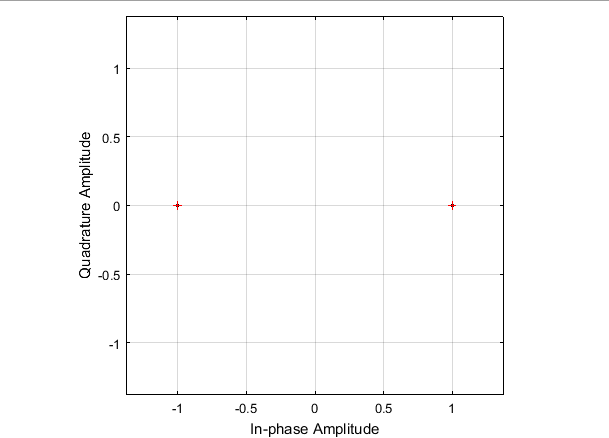
\includegraphics[width=\linewidth]{ConstelaBinSR.png}
\caption{Constelação Obtida sem Ruído}
\end{figure}
\pagebreak
\subsection{Com Ruído}
\begin{figure}
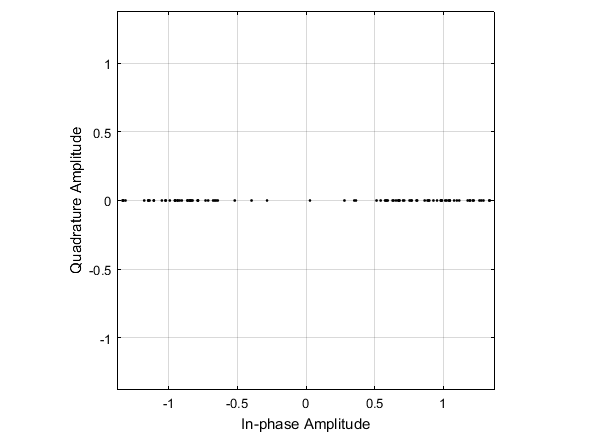
\includegraphics[width=\linewidth]{ConstelaBin10.png}
\caption{Constelação Obtida com Eb/No = 10dB}
\end{figure}
\begin{figure}
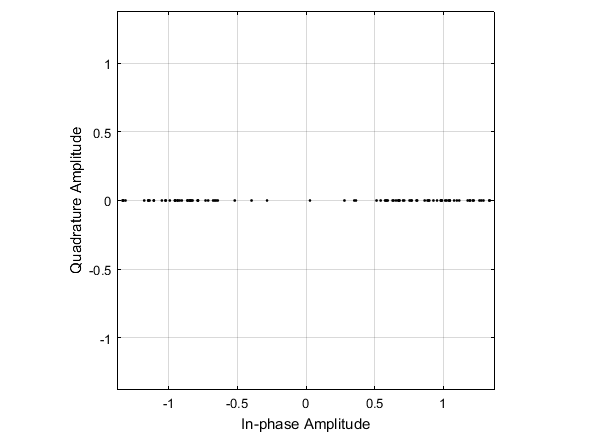
\includegraphics[width=\linewidth]{ConstelaBin10.png}
\caption{Constelação Obtida com Eb/No = 5dB}
\end{figure}
\pagebreak
\section{Taxa de Erro de Bit e Probabilidade de Erro}
É possível ver que para um certo número de bits transmitidos a BER calculada difere um pouco do que seria esperado para a função Q. Este comportamento é esperado pois a natureza estocástica do erro de bit fará com que a medida que aumentamos o número de bits transmitidos usados para calcular a BER, tenhamos um comportamento mais próximo à curva estudada em sala. Em geral temos um pouco mais ou menos erros de bits do que o centro da média que seria a função Q, como transmitimos poucos bits, cada erro terá um peso maior no cálculo da BER, desta forma observamos uma grande flutuação para poucos bits transmitidos e uma flutuação menor para muitos bits pois cada erro individualmente conta menos para o cálculo da BER.\\

É claramente observável que a medida que melhoramos a relação entre a energia transmitida e o ruído, a BER cai. De acordo com o que estudamos em sala.\\
\begin{figure}
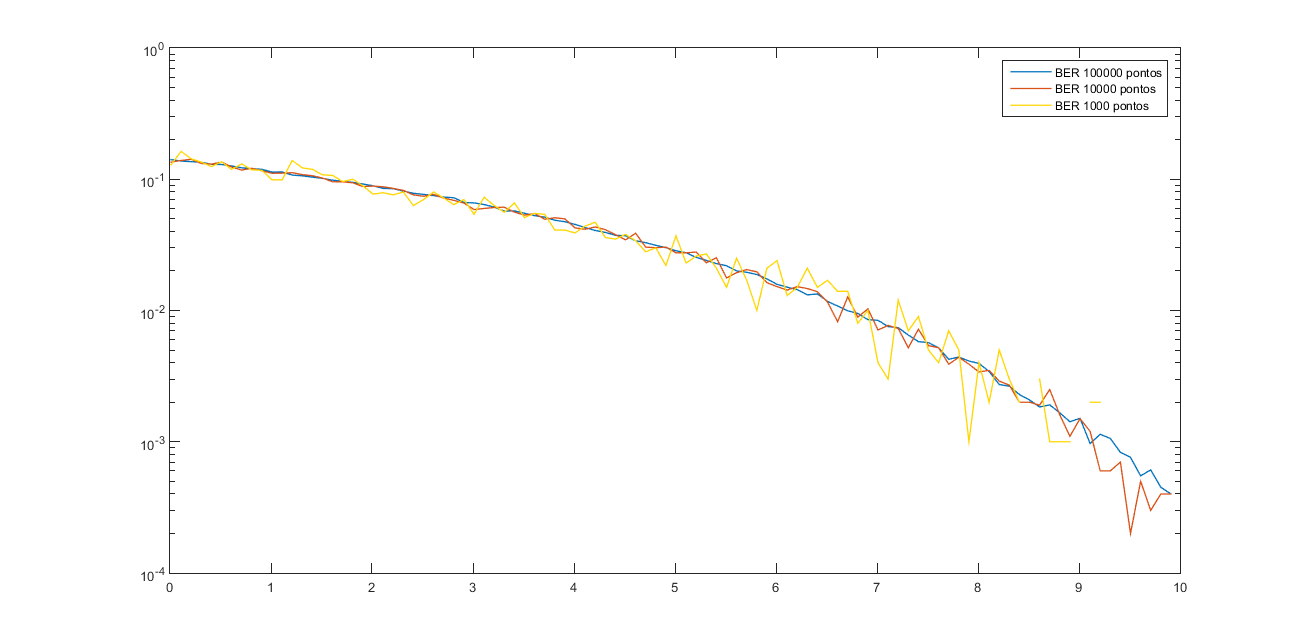
\includegraphics[width=\linewidth]{BERfigura.png}
\caption{Taxas de Erro de Bit para Eb/No em incrementos de 0.1}
\end{figure}
\end{document}         